\documentclass[12pt,a4paper]{article}

\usepackage[a4paper,margin=1in]{geometry}
\usepackage[T1]{fontenc}
\usepackage[utf8]{inputenc}
\usepackage{graphicx}
\usepackage{lmodern}
\usepackage{parskip}
\usepackage[hidelinks]{hyperref}
\usepackage{enumitem}
\usepackage{subcaption}
\usepackage{float}
\usepackage{setspace}

\setstretch{1.05}
\setlist[itemize]{leftmargin=1.5em}

\title{\textbf{Personal Reflection Report}\\Panda Scooter Project}
\author{Zhicheng Zhang}
\date{}

\begin{document}
\maketitle

\section*{1. Role and Scope}

At the start of the project, my primary Belbin role was the \textbf{Shaper (SH)}. In practice, I worked as a \textbf{frontend engineer} and a \textbf{product manager}. My concrete responsibility was to deliver the \textbf{user app} and the \textbf{dispatcher app}, and I learned \textbf{uni-app} quickly so I could work across both frontend codebases.

The Shaper role fit my working style well. I tended to push the team to turn abstract ideas into concrete deliverables and to keep the project moving. In this project, that meant translating requirements into pages, confirming interfaces with the backend team, and making sure the frontend work stayed aligned with the overall product direction.

The first example was the early requirement and prototype stage. I helped clarify the workflows for scooter discovery, unlock and lock operations, ride tracking, and map-based management. I also participated in the wireframe discussion so the page structure was settled before implementation. This showed the Shaper role because I was actively driving the team from vague ideas to an executable plan.

The second example was the actual frontend delivery work. I implemented the rider-side pages and the dispatcher-side pages, and I used my prior frontend experience to learn uni-app quickly. This allowed me to switch between the two apps without slowing the team down. It also showed that I could take responsibility for real deliverables rather than only discuss requirements.



\section*{2. Key Contributions}

\subsection*{2.1 Requirement Understanding and Prototype Design}

I clarified requirements and page flows for three user groups (scooter discovery, unlock/lock, ride tracking, map management), reducing ambiguity and rework.

\begin{figure}[H]
  \centering
  \begin{subfigure}[t]{0.48\linewidth}
    \centering
    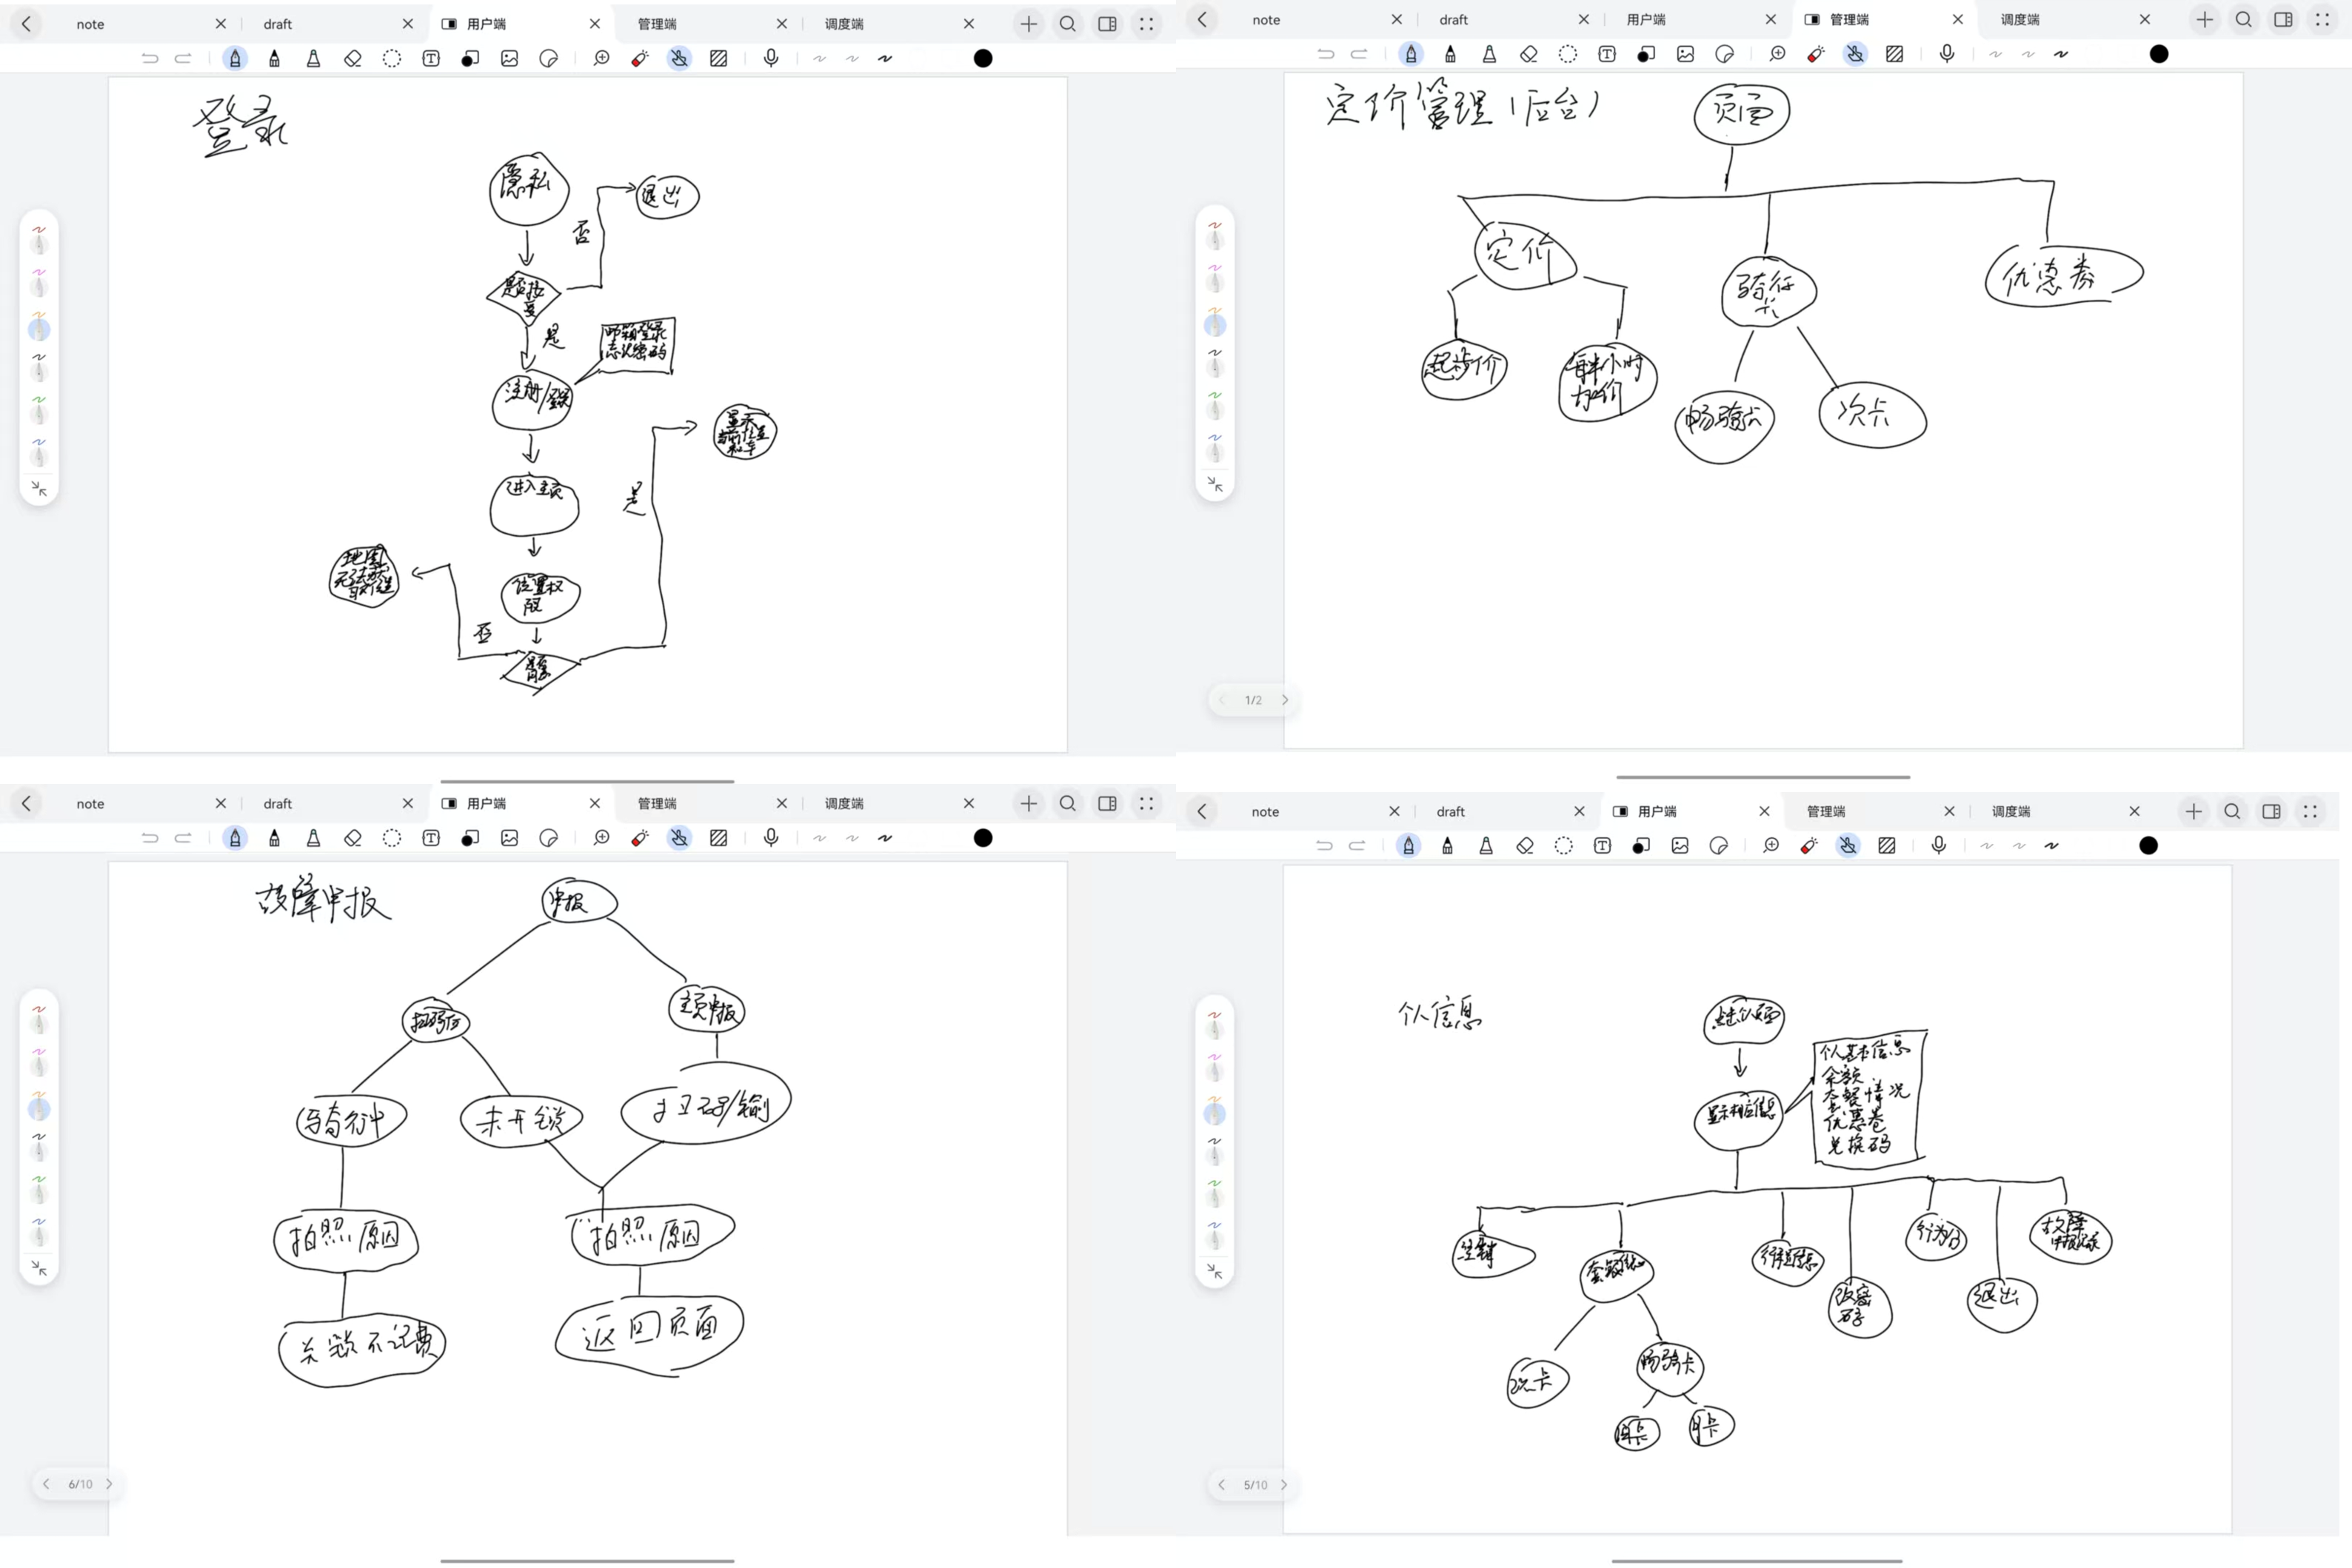
\includegraphics[width=\linewidth]{Early prototype discussion for the user flow.png}
    \caption{Early prototype discussion.}
  \end{subfigure}\hfill
  \begin{subfigure}[t]{0.48\linewidth}
    \centering
    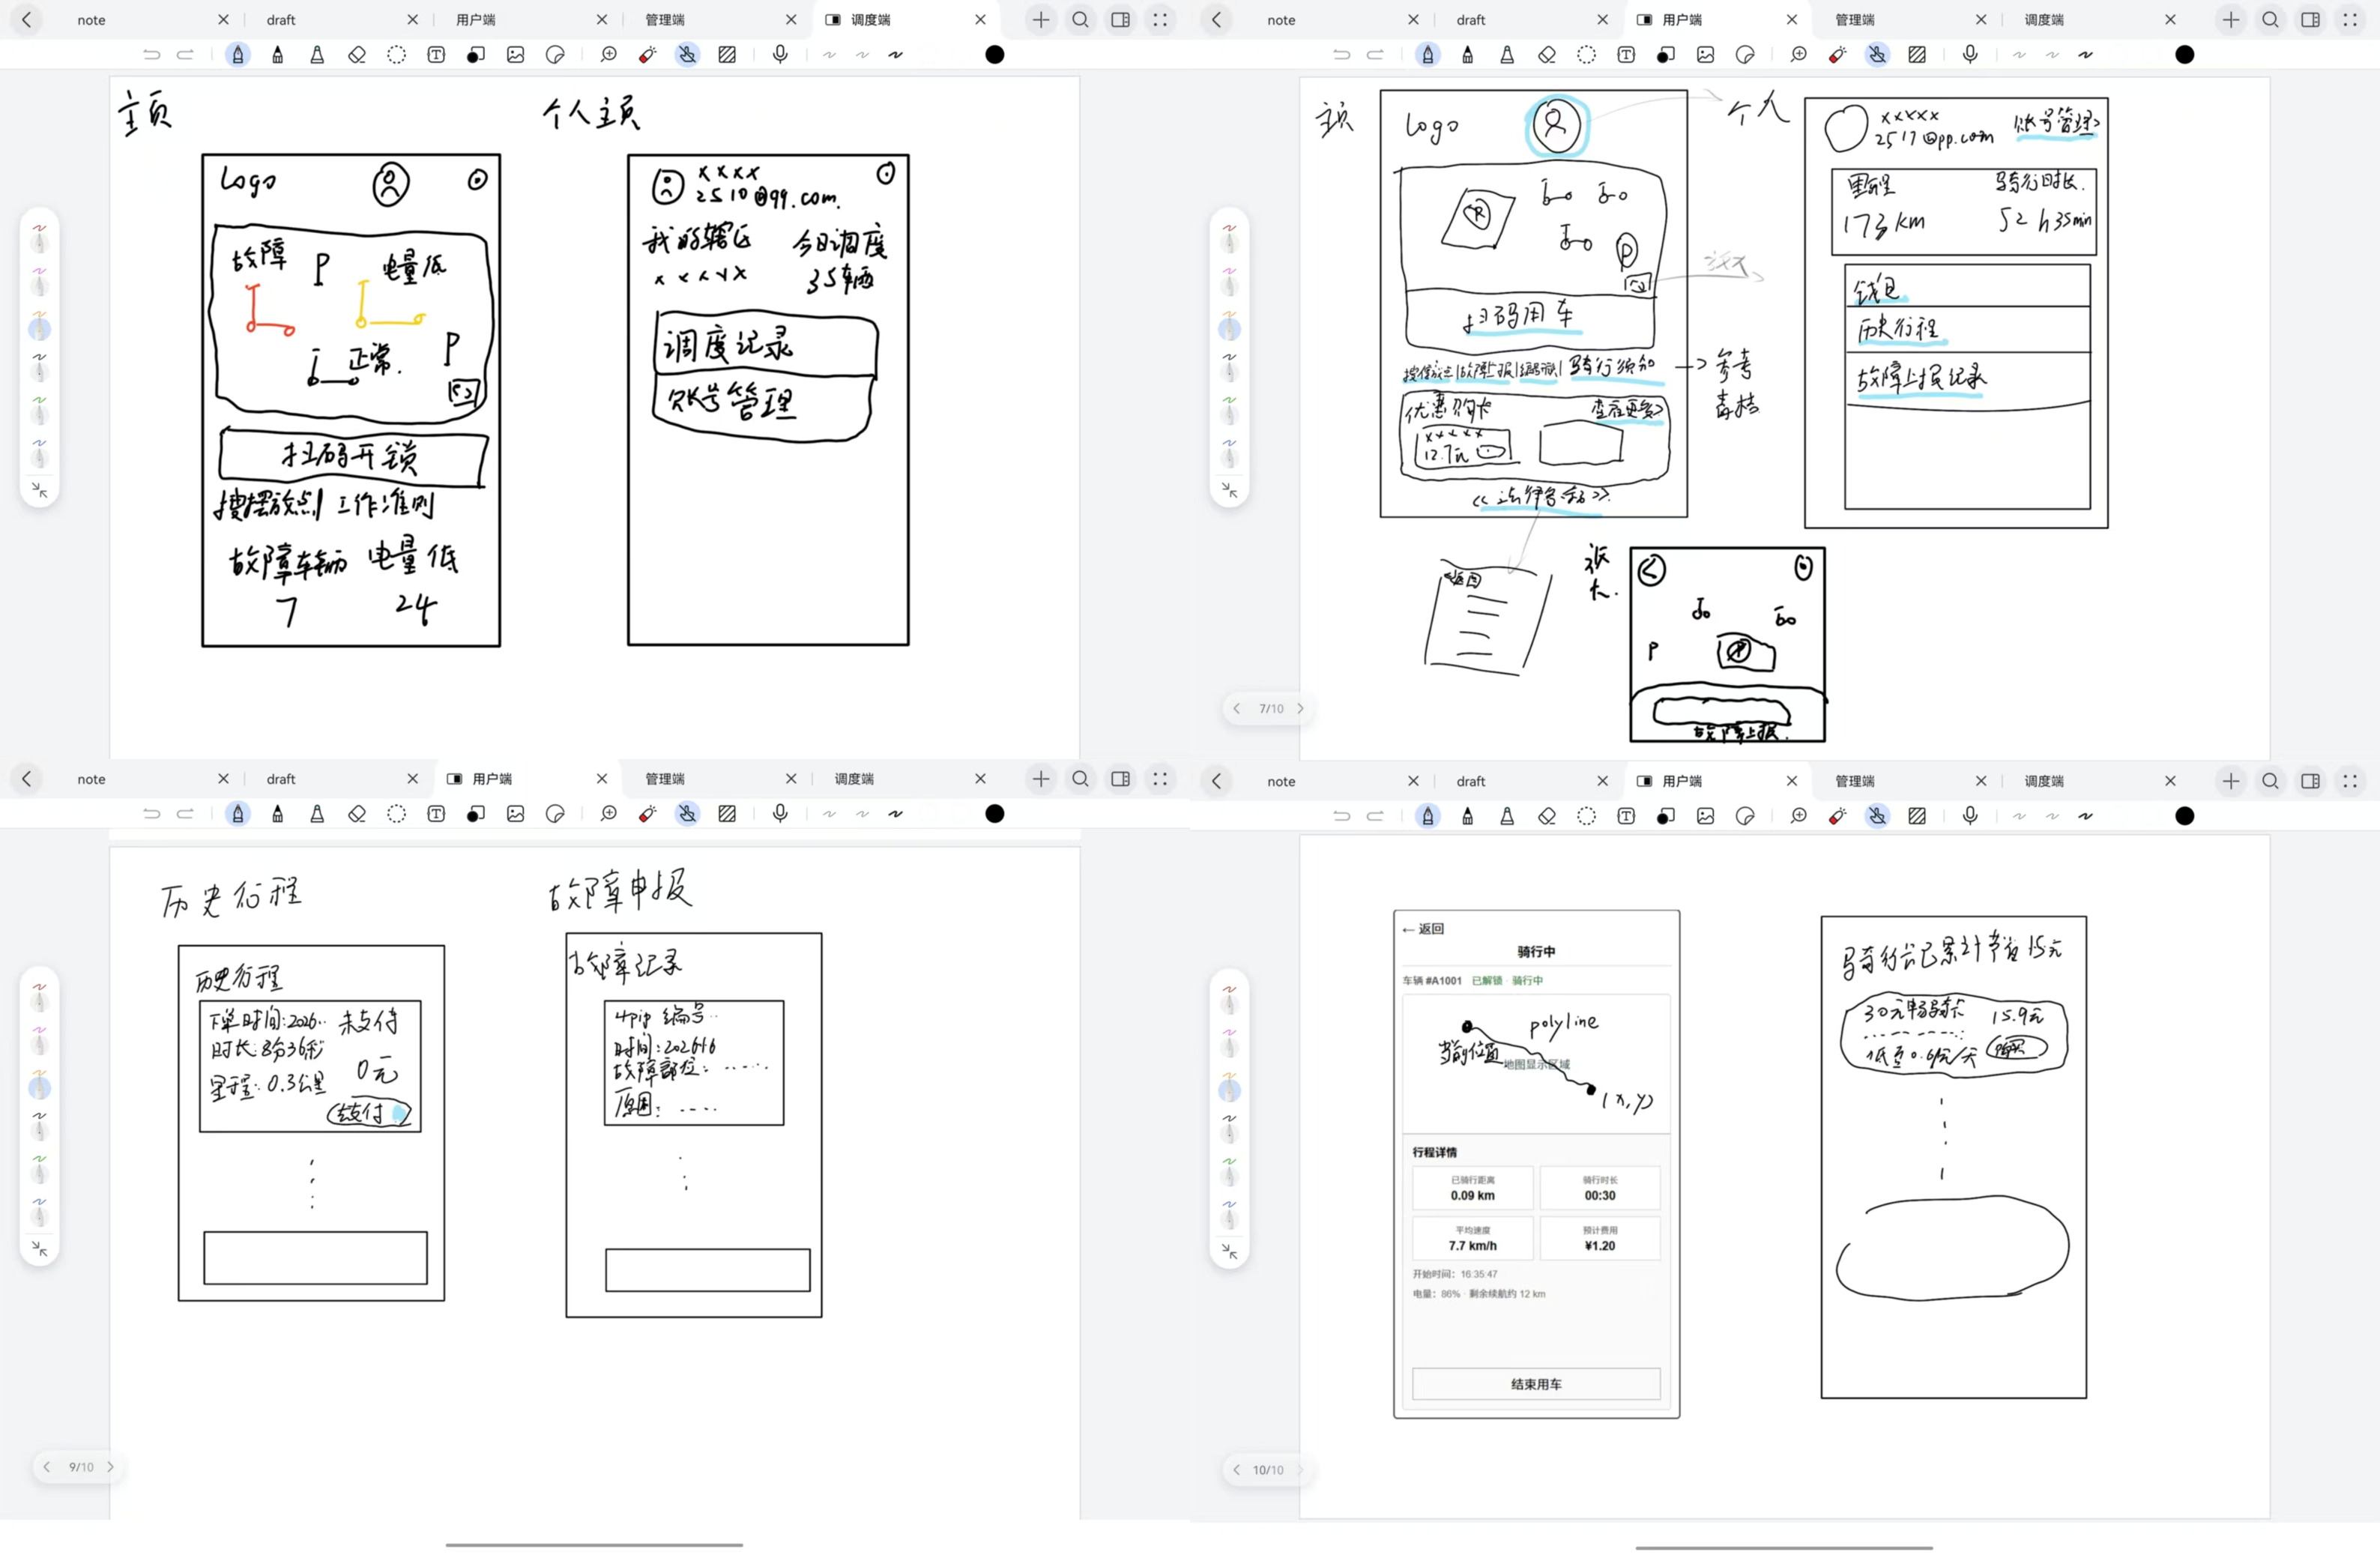
\includegraphics[width=\linewidth]{Wireframe or UI draft for the main riding workflow.png}
    \caption{Wireframe for the workflow.}
  \end{subfigure}
  \caption{Prototype discussion and wireframe used to define the main user flow.}
\end{figure}

\subsection*{2.2 API Collaboration}

To keep frontend and backend integration efficient, I used Apifox to align interface definitions and test the API before implementation.

\begin{figure}[H]
  \centering
  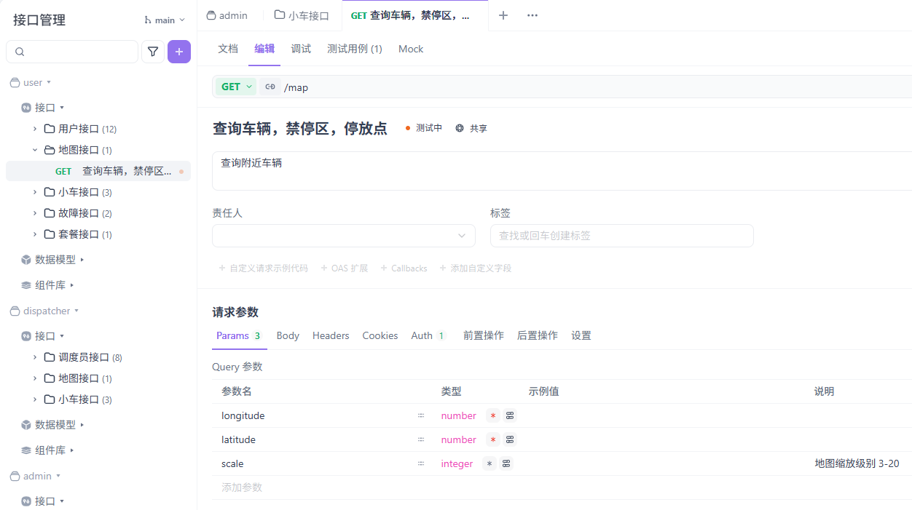
\includegraphics[width=0.92\linewidth]{API coordination in Apifox used for frontend-backend integration.png}
  \caption{API coordination in Apifox.}
\end{figure}

\subsection*{2.3 Frontend Delivery}

I translated the agreed design into the actual rider and dispatcher pages, making sure the two apps matched the intended workflow.

\begin{figure}[H]
  \centering
  \begin{subfigure}[t]{0.48\linewidth}
    \centering
    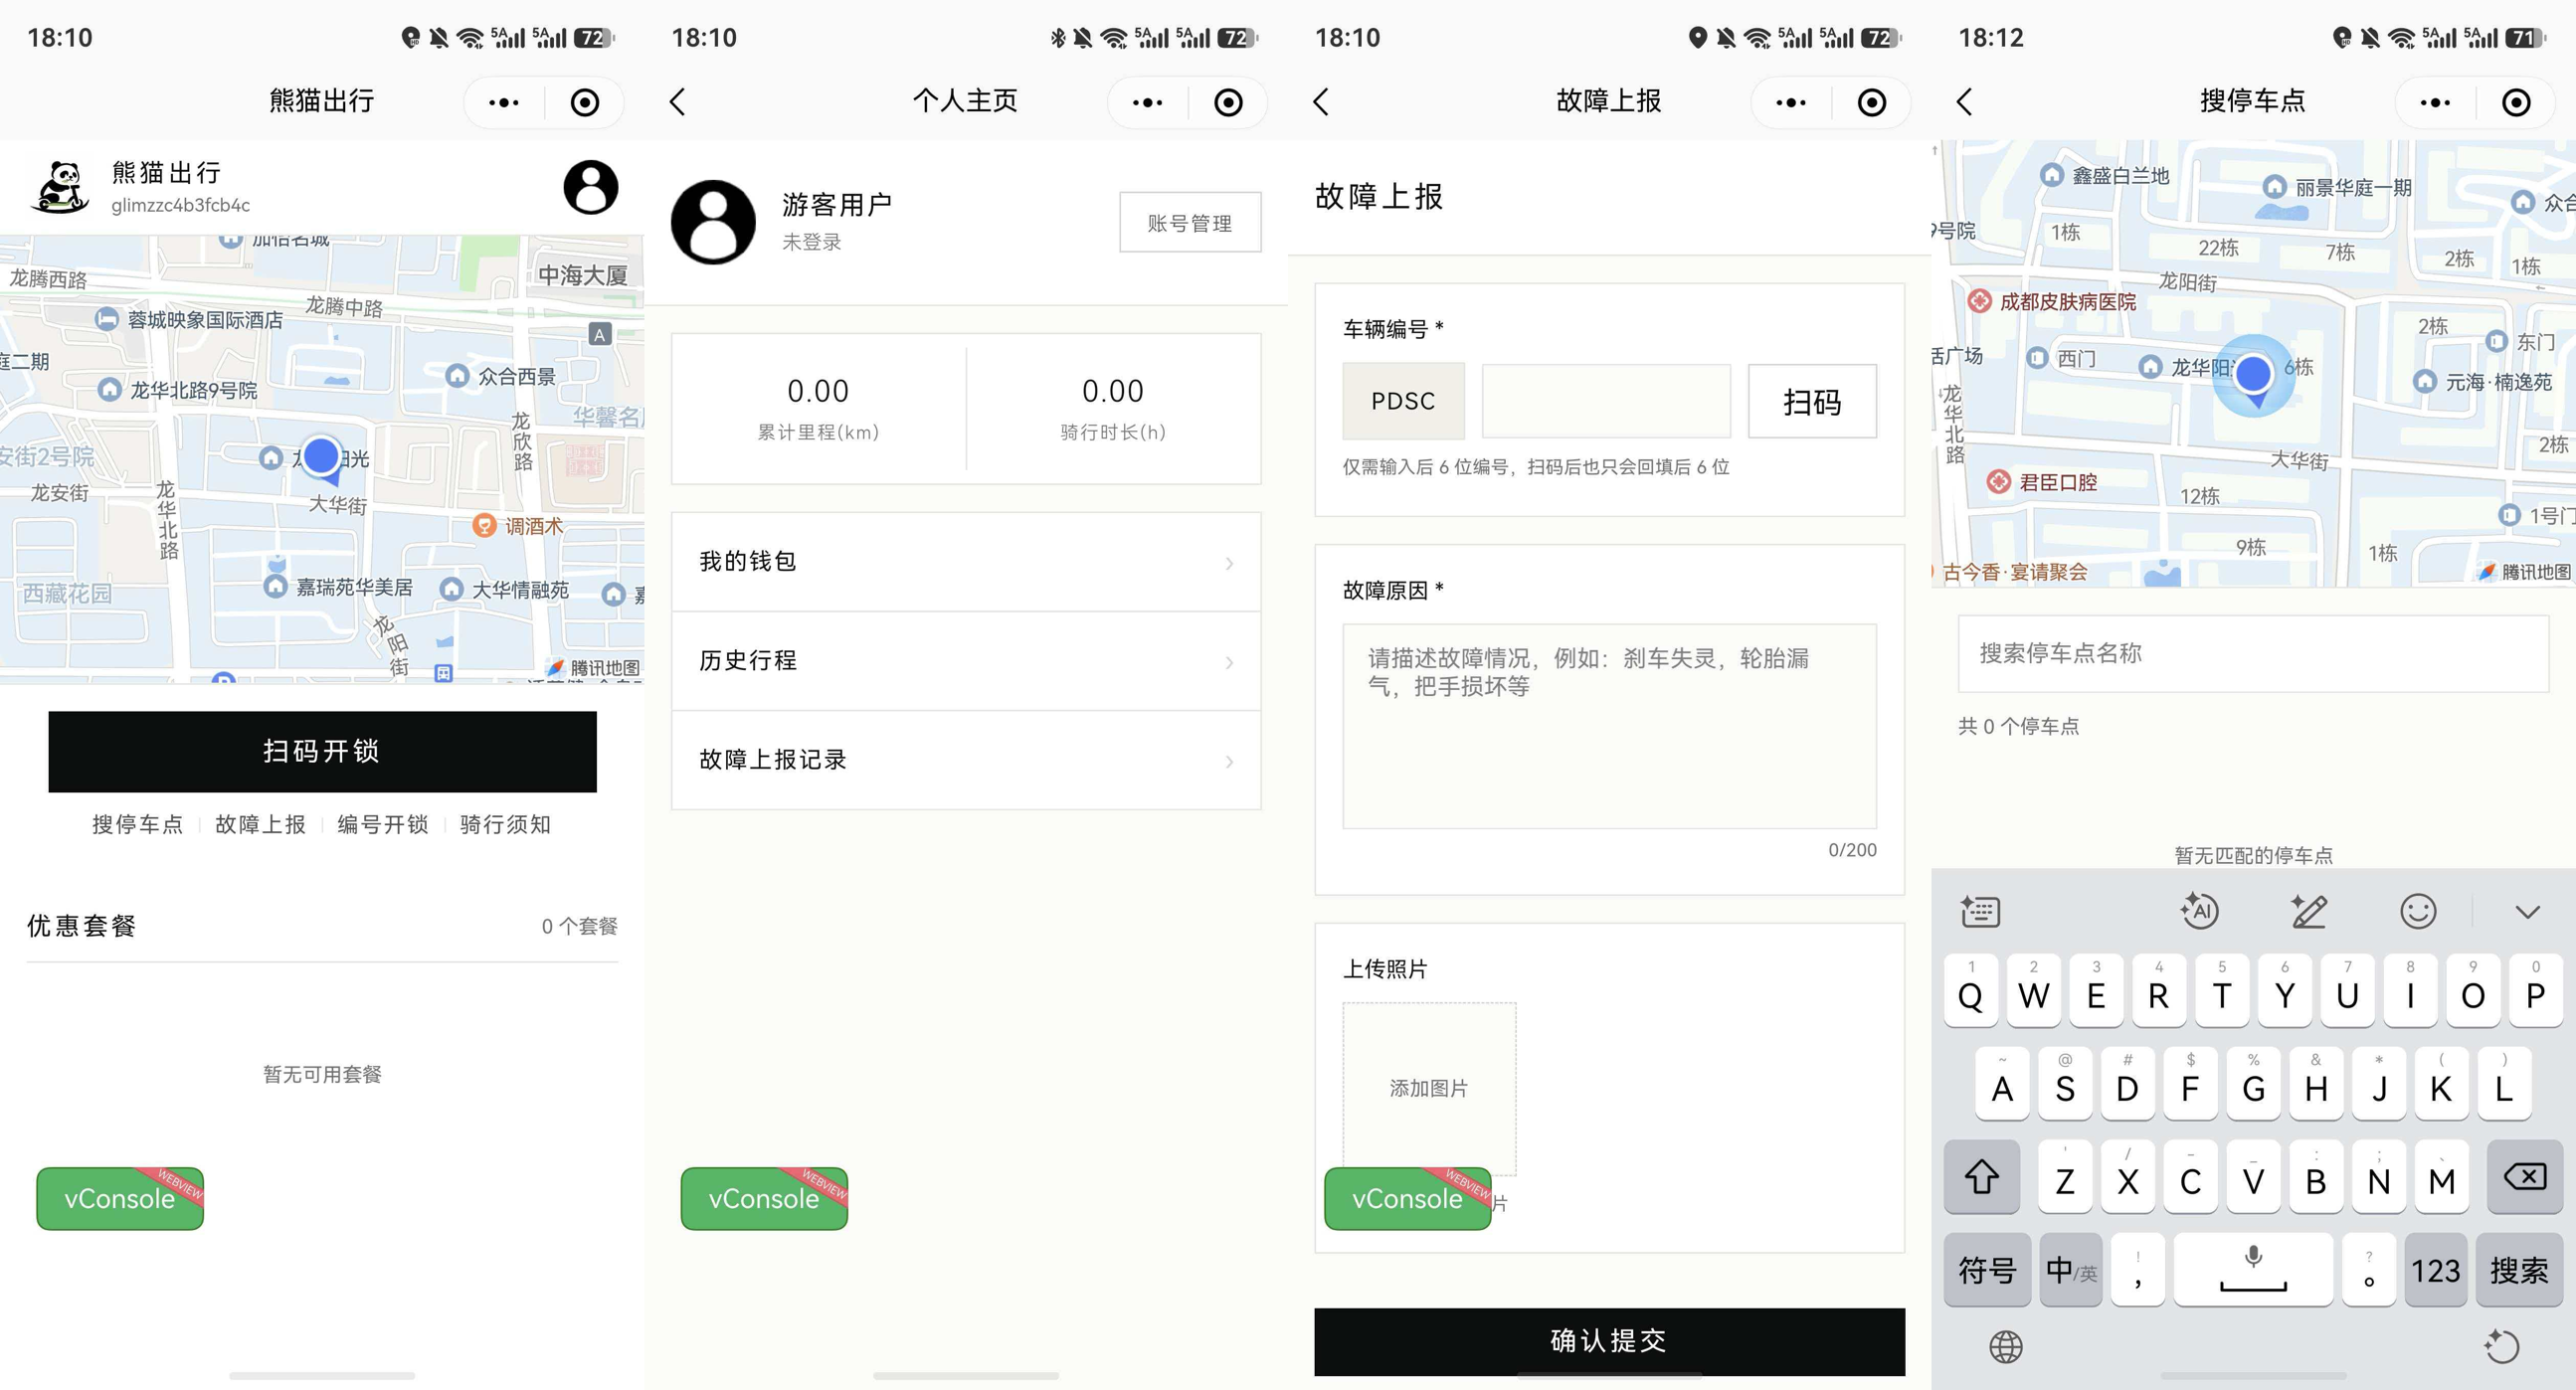
\includegraphics[width=\linewidth]{Main user interface implemented for the rider app.png}
    \caption{User-side pages.}
  \end{subfigure}\hfill
  \begin{subfigure}[t]{0.48\linewidth}
    \centering
    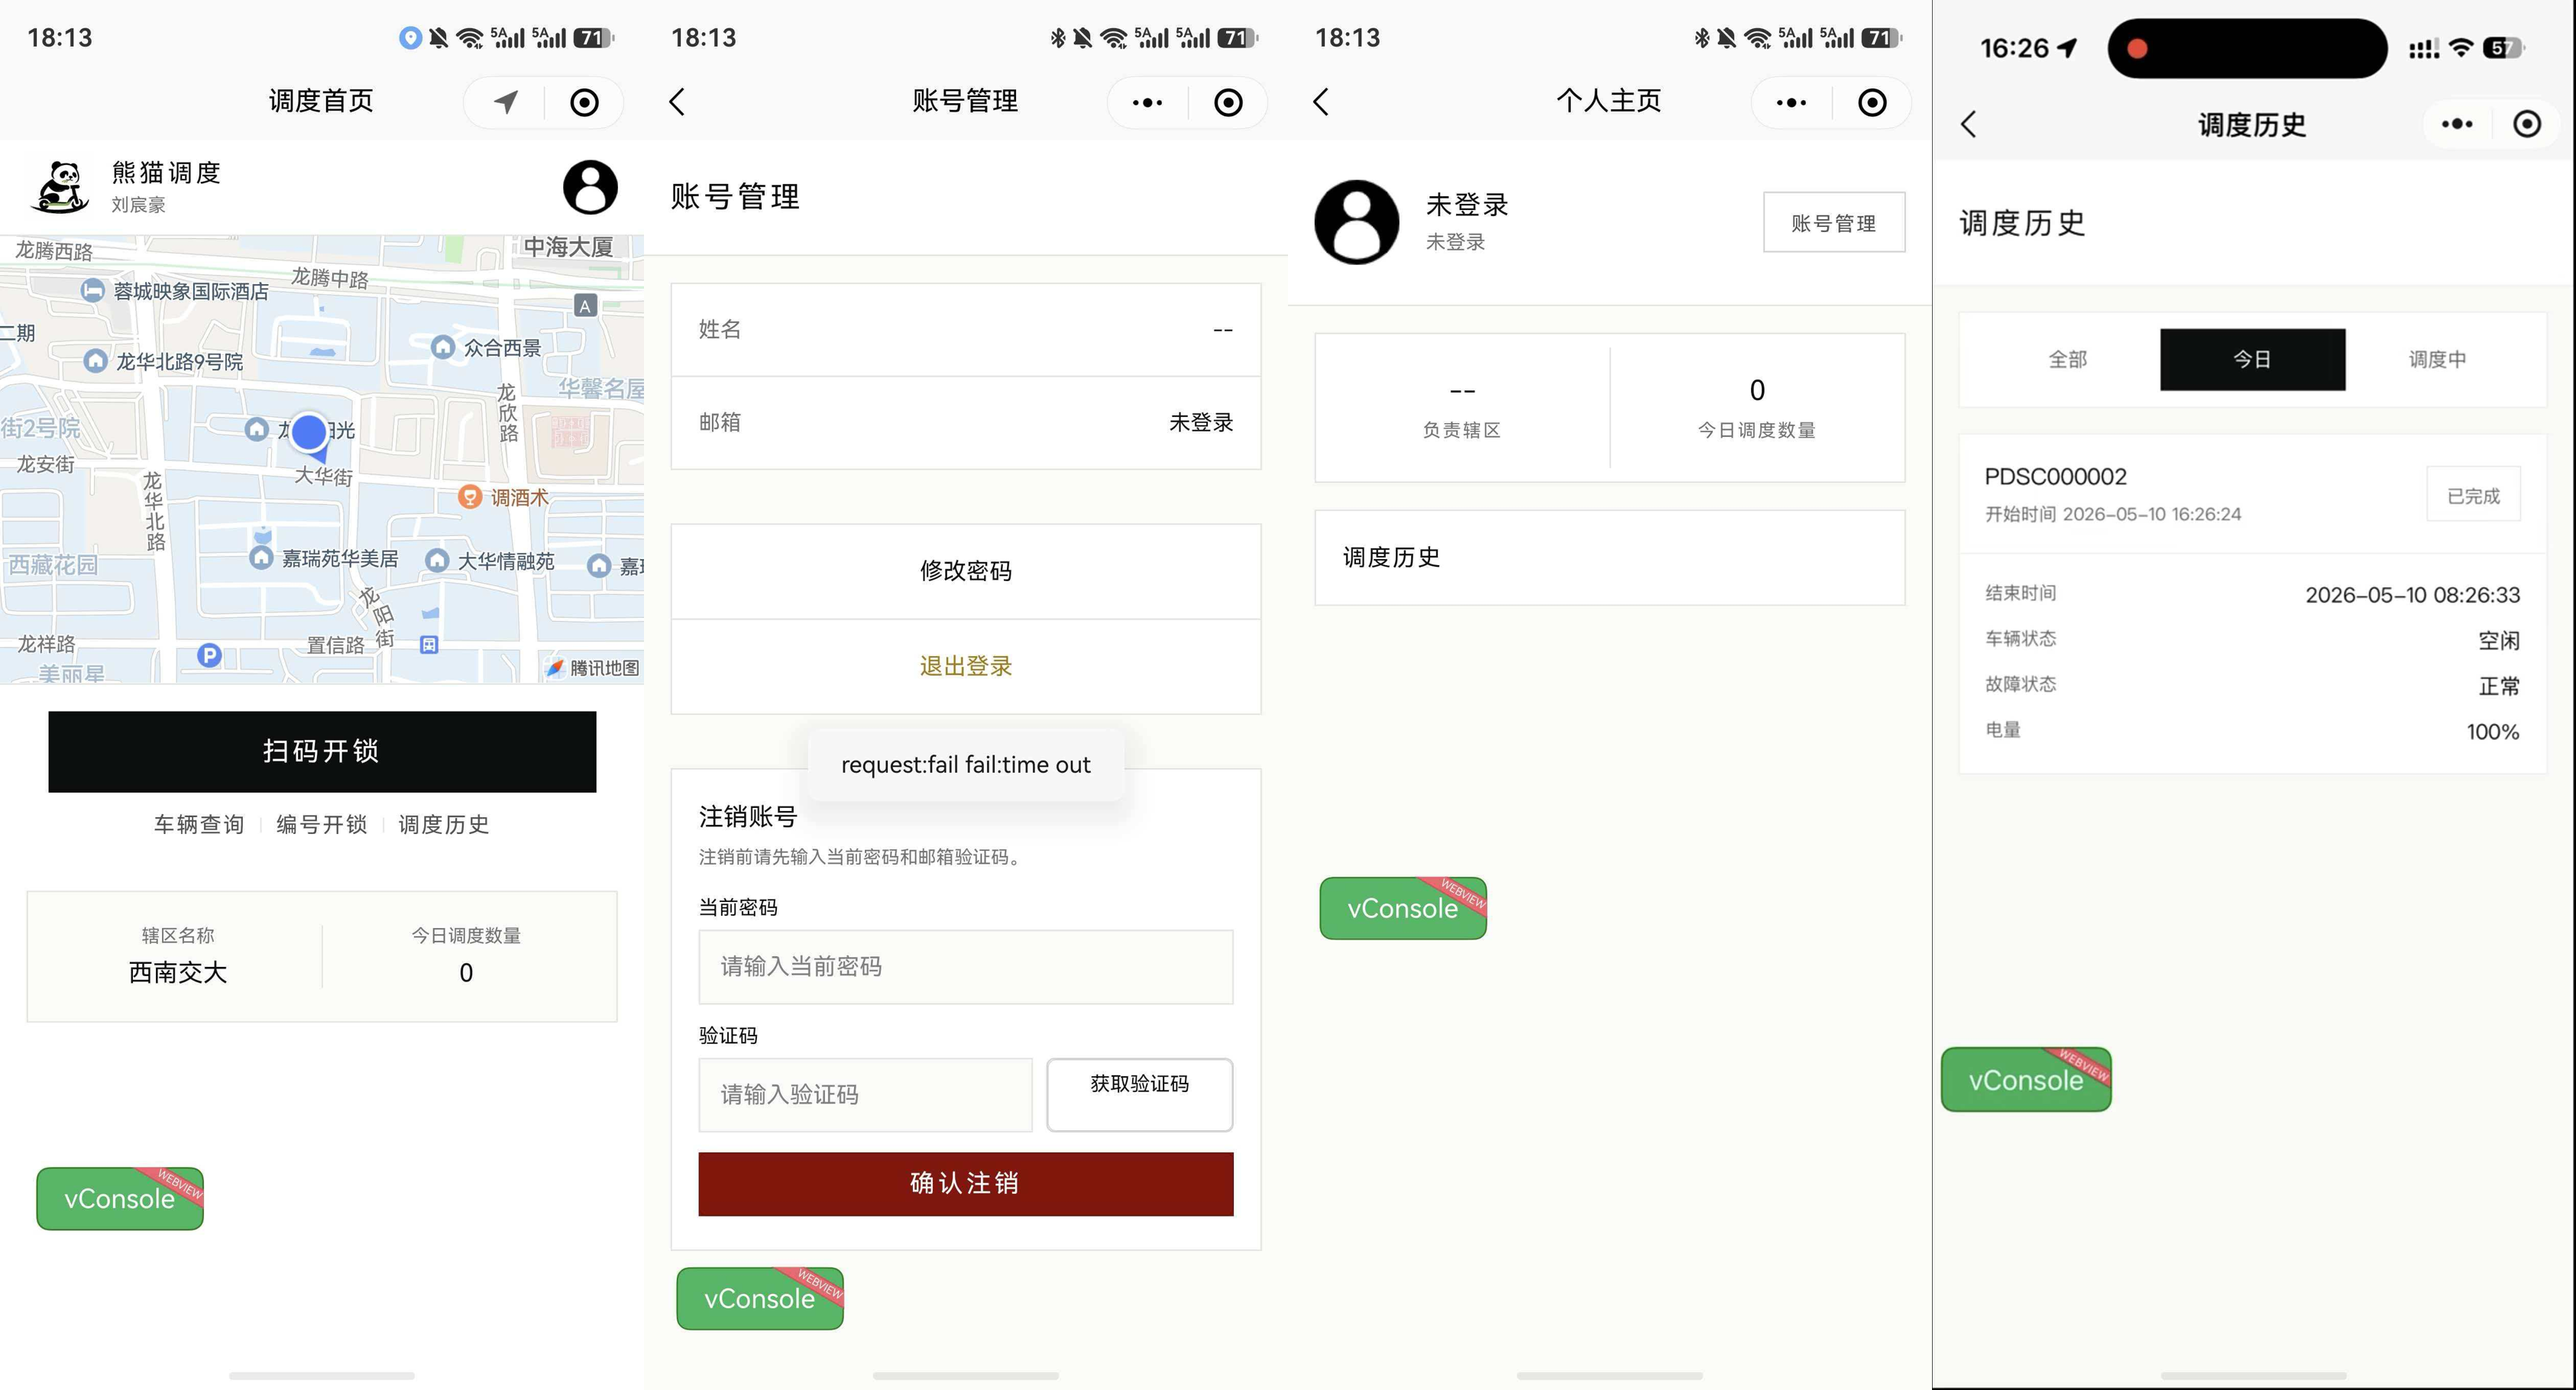
\includegraphics[width=\linewidth]{Dispatcher page developed during implementation.png}
    \caption{Dispatcher-side pages.}
  \end{subfigure}
  \caption{The two frontend applications I delivered as the frontend engineer.}
\end{figure}

\section*{3. Strengths}

Two strengths stood out in my role: \textbf{communication and adaptability}. Because I understood both product goals and implementation details, I could explain user needs clearly to the team and turn technical constraints back into practical interface decisions.

The first part of this strength was my ability to handle early-stage design thinking. Before implementation, I helped the team discuss the user flow and the wireframe, so the interface direction was clear before code writing started. This improved team alignment and reduced repeated changes.

Another strength was \textbf{frontend framework experience and fast learning}. Since I had experience on frontend framework like Vue and React, I learned \textbf{uni-app} quickly and became productive across both frontend codebases in a short time. That helped the team keep momentum during implementation because I could contribute to two separate frontend streams without a long ramp-up period.

\begin{figure}[H]
  \centering
  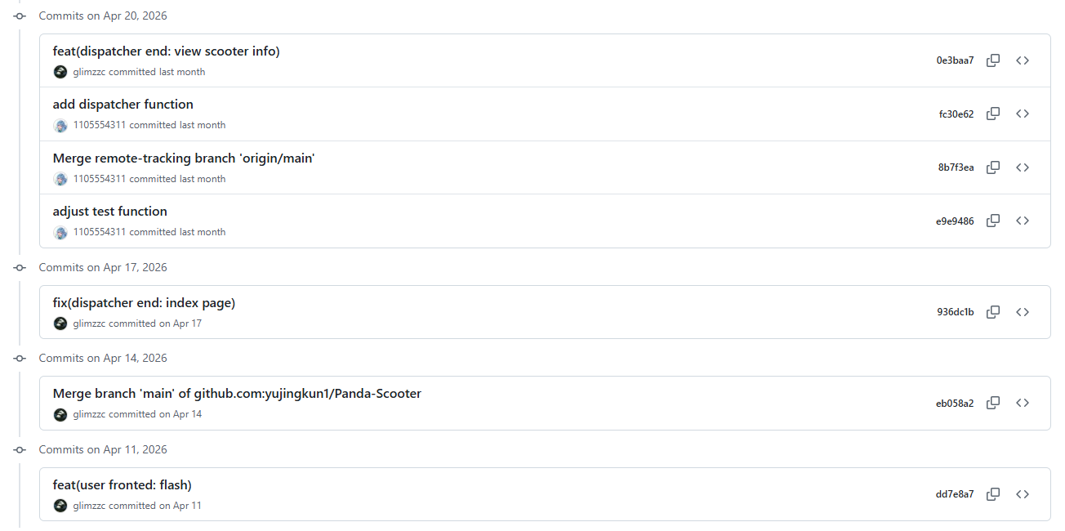
\includegraphics[width=0.92\linewidth]{Github commitment records.png}
  \caption{GitHub commit history showing that I ramped up quickly and delivered iteratively across tasks.}
\end{figure}

\section*{4. Weaknesses and Improvement}

My first weakness was that, as a frontend engineer, my UI design ability was not as polished as a dedicated designer's. The team had already produced wireframes, but I still had to make many concrete UI decisions during implementation. That meant some visual design work was left to me at the coding stage, and the division of work was not ideal. To deal with this, I used the wireframes as a baseline and kept the UI simple and consistent instead of trying to redesign the whole interface.

My second weakness was that my task load was too broad. I had to complete coding work while also participating in increasing requirement implementation planning, so I could not focus on one area completely. This sometimes split my attention between design, development, and coordination, which affected efficiency and made me switch context more often than I should have. I dealt with this by using short communication cycles, confirming requirements before coding, and breaking the work into smaller steps.

Overall, these weaknesses showed that I was effective in delivery, but I still needed better balance between visual design, implementation, and planning.

\begin{figure}[H]
  \centering
  \includegraphics[width=0.92\linewidth]{GitHub wiki.png}
  \caption{GitHub wiki (Tasks involve requirement analysis, API document writing and pages implementation).}
\end{figure}

\end{document}
